\documentclass{article}
\usepackage[utf8]{inputenc}
\usepackage[T1]{fontenc}
\usepackage{amsmath}
\usepackage{graphicx}
\usepackage{listings}
\usepackage{xcolor}
\usepackage{makecell}
\usepackage{float}

\lstset{
	language=C++,
	backgroundcolor=\color{black!5},
	basicstyle=\footnotesize\ttfamily,
	keywordstyle=\color{blue},
	commentstyle=\color{green!50!black},
	stringstyle=\color{red!70!black},
	numbers=left,
	numberstyle=\tiny\color{gray},
	stepnumber=1,
	frame=single,
	rulecolor=\color{black!30},
	tabsize=4,
	breaklines=true,
	breakatwhitespace=false,
	showspaces=false,
	showstringspaces=false,
	showtabs=false
}

\title{Analiza i porównanie algorytmów sortowania}
\author{Tomasz Warzecha}


\begin{document}
	
	\maketitle
	
	\section{Wstęp}
W sprawozdaniu moim celem jest analiza i porównanie wydajności trzech algorytmów sortowania wraz z ich modyfikacjami. Quick sort, bucket sort, radix sort zostały zaimplementowane, tak aby przeprowadzić na nich różne testy wydajności. Badania te skupiają się na generowaniu losowych danych, które następnie są używane do obliczenia czasu wykonania algorytmów. Wyniki tych testów mają na celu porównanie algorytmów, a także pokazanie różnic między teoretycznymi, a praktycznymi wynikami. 
	
	\section{Implementacja algorytmów}
Algorytmy zostały zaimplementowane zgodnie z klasycznymi wersjami algorytmów sortujących, korzystając z pseudokodów zamieszczonych na stronie przez prof. Szymona Żeberskiego. Wprowadzone zostały także modyfikacje, które delikatnie zmieniają działanie algorytmów. Algorytmy quick sort oraz bucket zostały zaimplementowane dla tablic z liczbami typu \texttt{float}, natomiast radix sort - \texttt{int}.
	
	\paragraph{Najciekawsze fragmenty kodu\\}
	Poniżej przedstawię najciekawsze fragmenty kodu, wraz z objaśnieniami, tak aby łatwiej zrozumieć działanie algorytmów. 
	
	\subsection{\textit{Radix sort}}
	Do sortowania w sortowaniu pozycyjnym potrzebujemy dodatkowego algorytmu sortującego - w tym wypadku użyliśmy sortowania przez zliczanie. Sortowanie pozycyjne iteruje przez kolejne cyfry liczb w ustalonej podstawie, a następnie sortuje tablice względem danej cyfry za pomocą counting sort.
	\begin{lstlisting}
for (int poz = 1; max / poz > 0; poz *= baza) {
	coutingSort(A, n, baza, poz);
}
	\end{lstlisting}
	Funkcja \texttt{coutingSort} stabilnie sortuje nasze liczby według ustalonej cyfry. Robi to za pomocą dzielenia całkowitego i reszty z dzielenia przez podstawę systemu liczbowego:
	\begin{lstlisting}
int znak = (A[i] / poz) % baza;
B[C[znak] - 1] = A[i];
C[znak]--;
	\end{lstlisting}
	
	\subsection{\textit{Quick sort}}
	Sortowanie szybkie wykorzystuje strategię dziel i zwyciężaj. Wybieramy nasz pivot(w tym wypadku ostatni element) i za pomocą funkcji partition dzielimy tablicę na dwie części - liczby mniejsze od wartości pivota i większe od niej:
	\begin{lstlisting}
void quickSort(float A[],int p, int k){
	if(p < k){
		int s = partition(A,p,k);
		quickSort(A,p,s-1);
		quickSort(A,s+1,k);
	}
}
		
	\end{lstlisting}
	
	\subsection{\textit{Bucket sort}}
	Sortowanie kubełkowe grupuje dane w przedziały(kubełki), a następnie wewnątrz nich stosuje dodatkowe sortowanie (w tym wypadku insertion sort). Posortowane kubełki złącza w następujący sposób w naszą posortowaną listę.
	\begin{lstlisting}
for(int j=0;j<n;j++){
	for(int k =0; k<dlugosci[j]; k++){
		A[i] = B[j][k];
		i++;
	}
}
	\end{lstlisting}
	
	\section{Porównanie algorytmów}
	
	\subsection{Porównanie teoretyczne}
	Poniżej zestawiono złożoności czasowe, stabilność oraz złożoność pamięciową dla klasycznych wersji algorytmów:
	\begin{table}[H]
		\begin{tabular}{|l|c|c|c|c|}
			\hline
			\textbf{Algorytm}       & \textbf{Optymistyczna} & \textbf{Pesymistyczna}  & \textbf{Pamięciowa} & \textbf{Stabilność} \\ \hline
			\textit{Radix sort}     & $O(nk)$                & $O(nk)$                & $O(n + k)$          & Tak                 \\ \hline
			\textit{Quick sort}     & $O(n \log n)$          & $O(n^2)$               & $O(\log n)$         & Nie                 \\ \hline
			\textit{Bucket sort}    & $O(n + k)$            & $O(n^2)$               & $O(n + k)$          & Tak                 \\ \hline
		\end{tabular}
		\caption{Porównanie teoretyczne algorytmów sortowania}
	\end{table}
	
	\subsection{Porównanie czasów działania}
	Zaprezentowano wyniki pomiarów na wykresach:
%	\begin{figure}[H]
		%\centering
		% 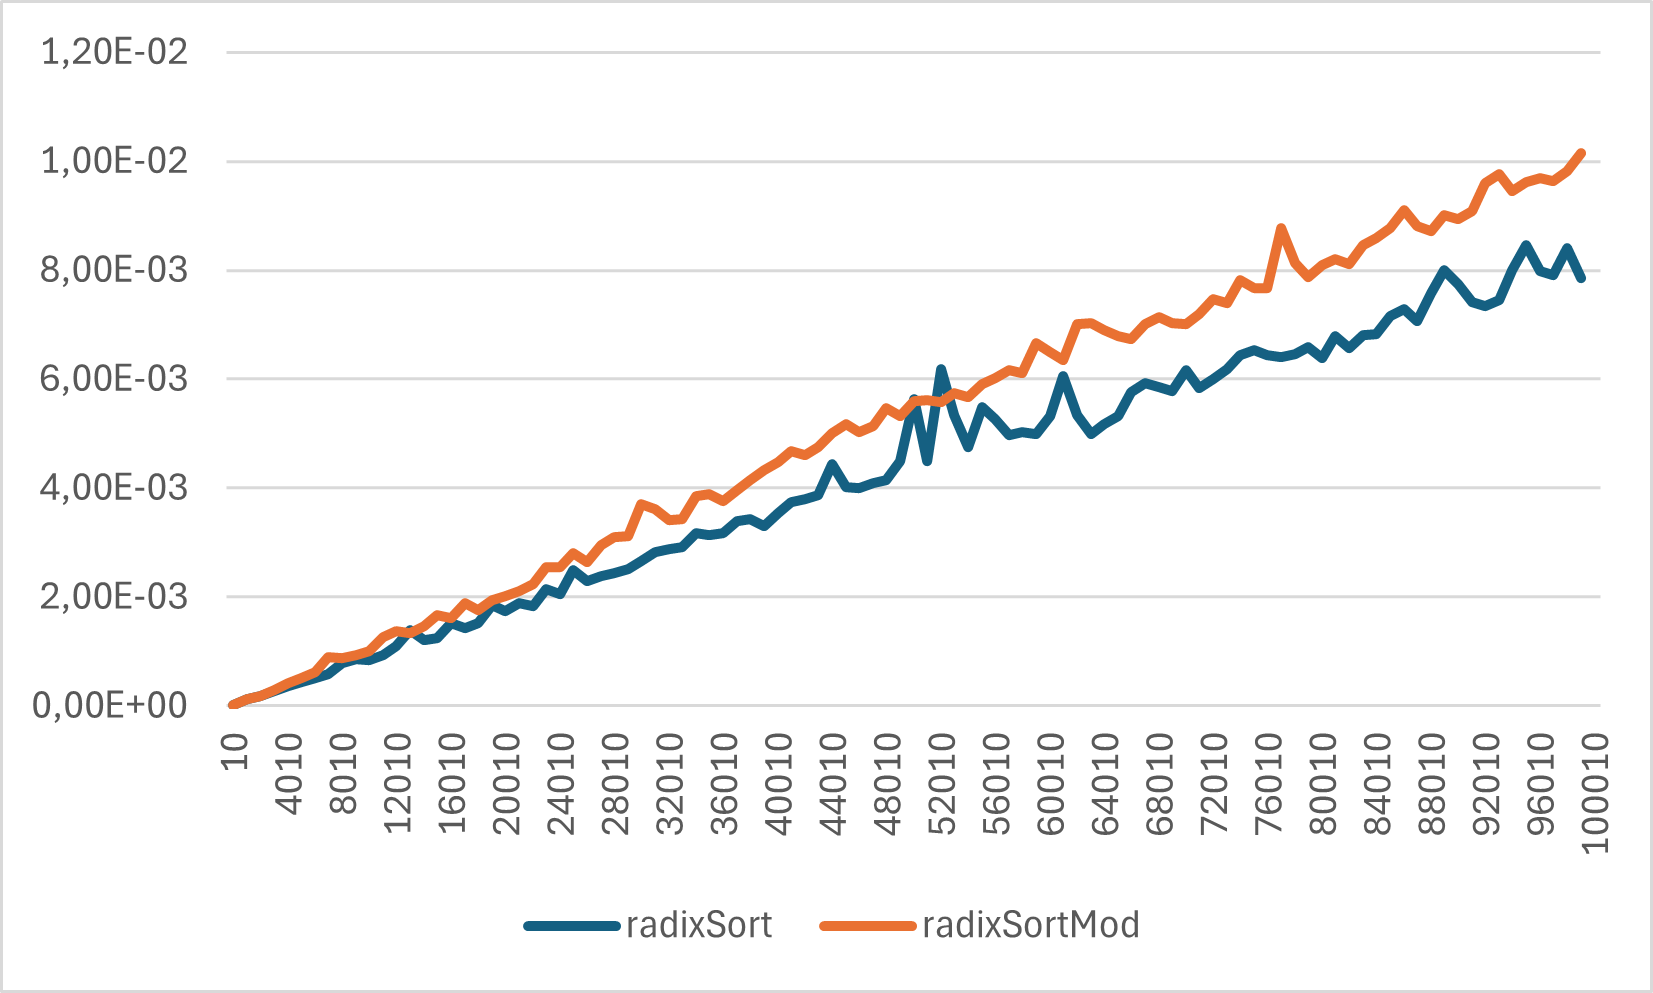
\includegraphics[width=\textwidth]{radix.png}
		%\caption{Czasy działania \textit{radix sort} w różnych podstawach}
%	\end{figure}
	
	\begin{figure}[H]
		\centering
		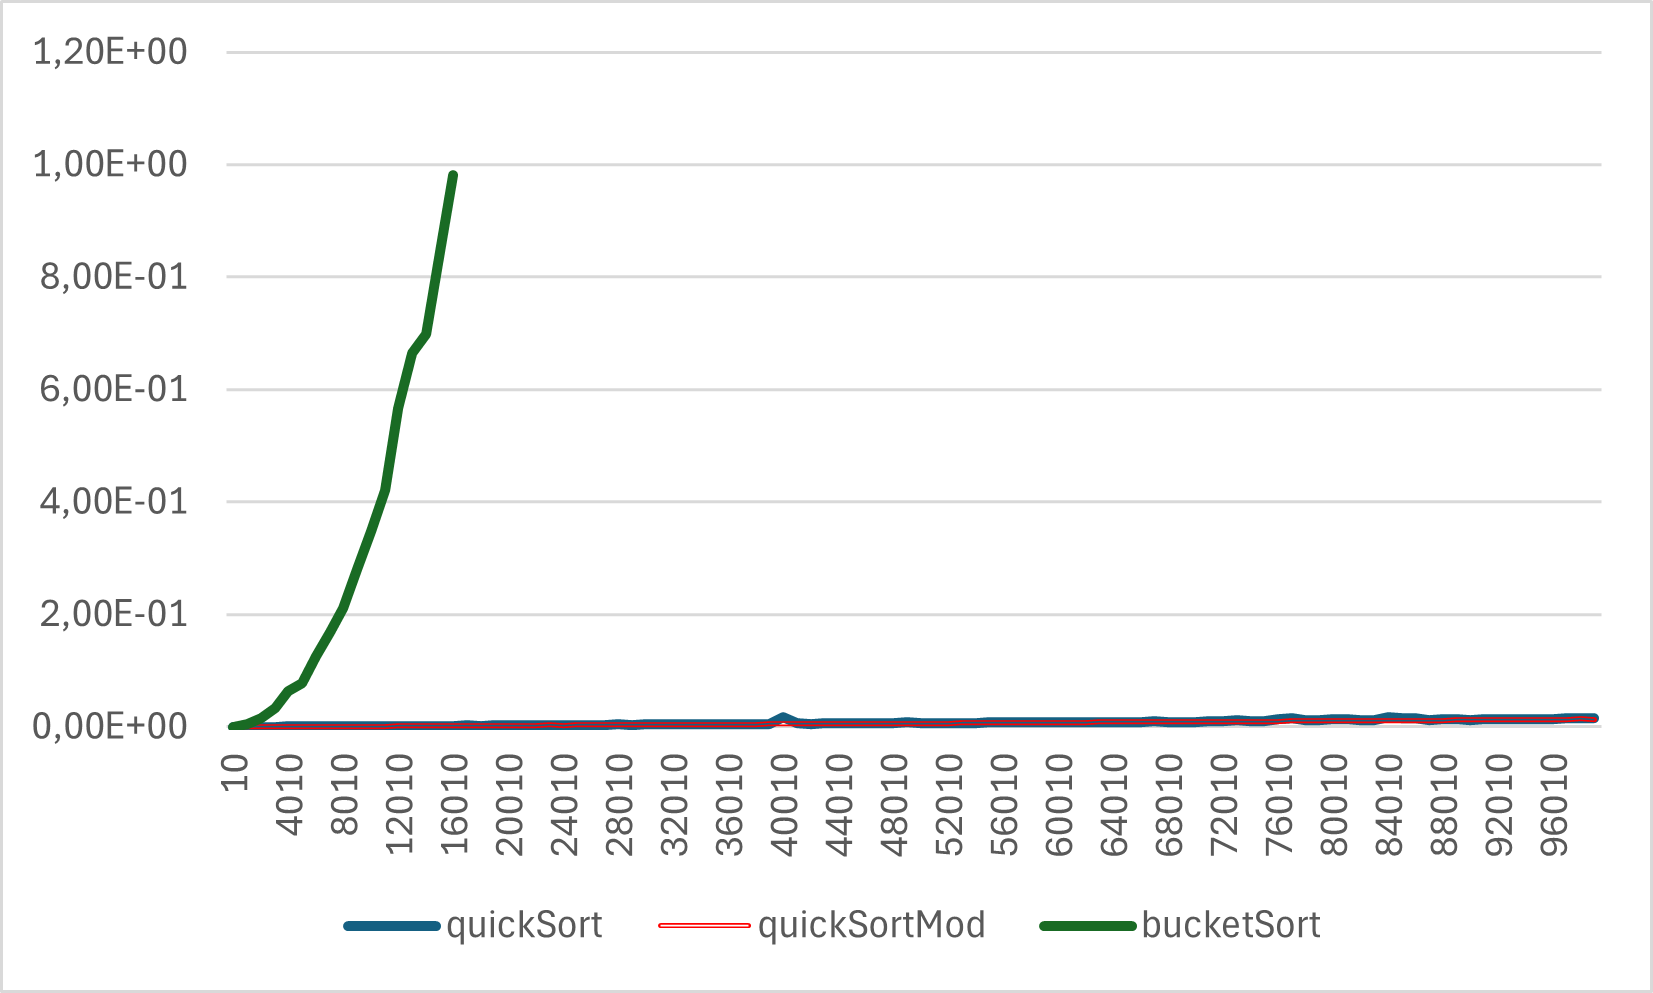
\includegraphics[width=\textwidth]{algorytmy.png}
		\caption{Porównanie czasów działania \textit{quick sort}, jego modyfikacji i \textit{bucket sort}}
	\end{figure}
	Na wykresie możemy zobaczyć, że quick sort jak i jego modyfikacja są znacząco szybsze. Jest to spowodowane dużo większą złożonością algorytmu sortowania kubełkowego. Natomiast możemy również zobaczyć, że nasza modyfikacja szybkiego sortowania znacząco nie zmieniła wyników. 
	
	\paragraph{Quick sort i radix sort}
	Porównamy teraz czasy działania dwóch podobnych złożeniowo algorytmów.
	\begin{figure}[H]
		\centering
		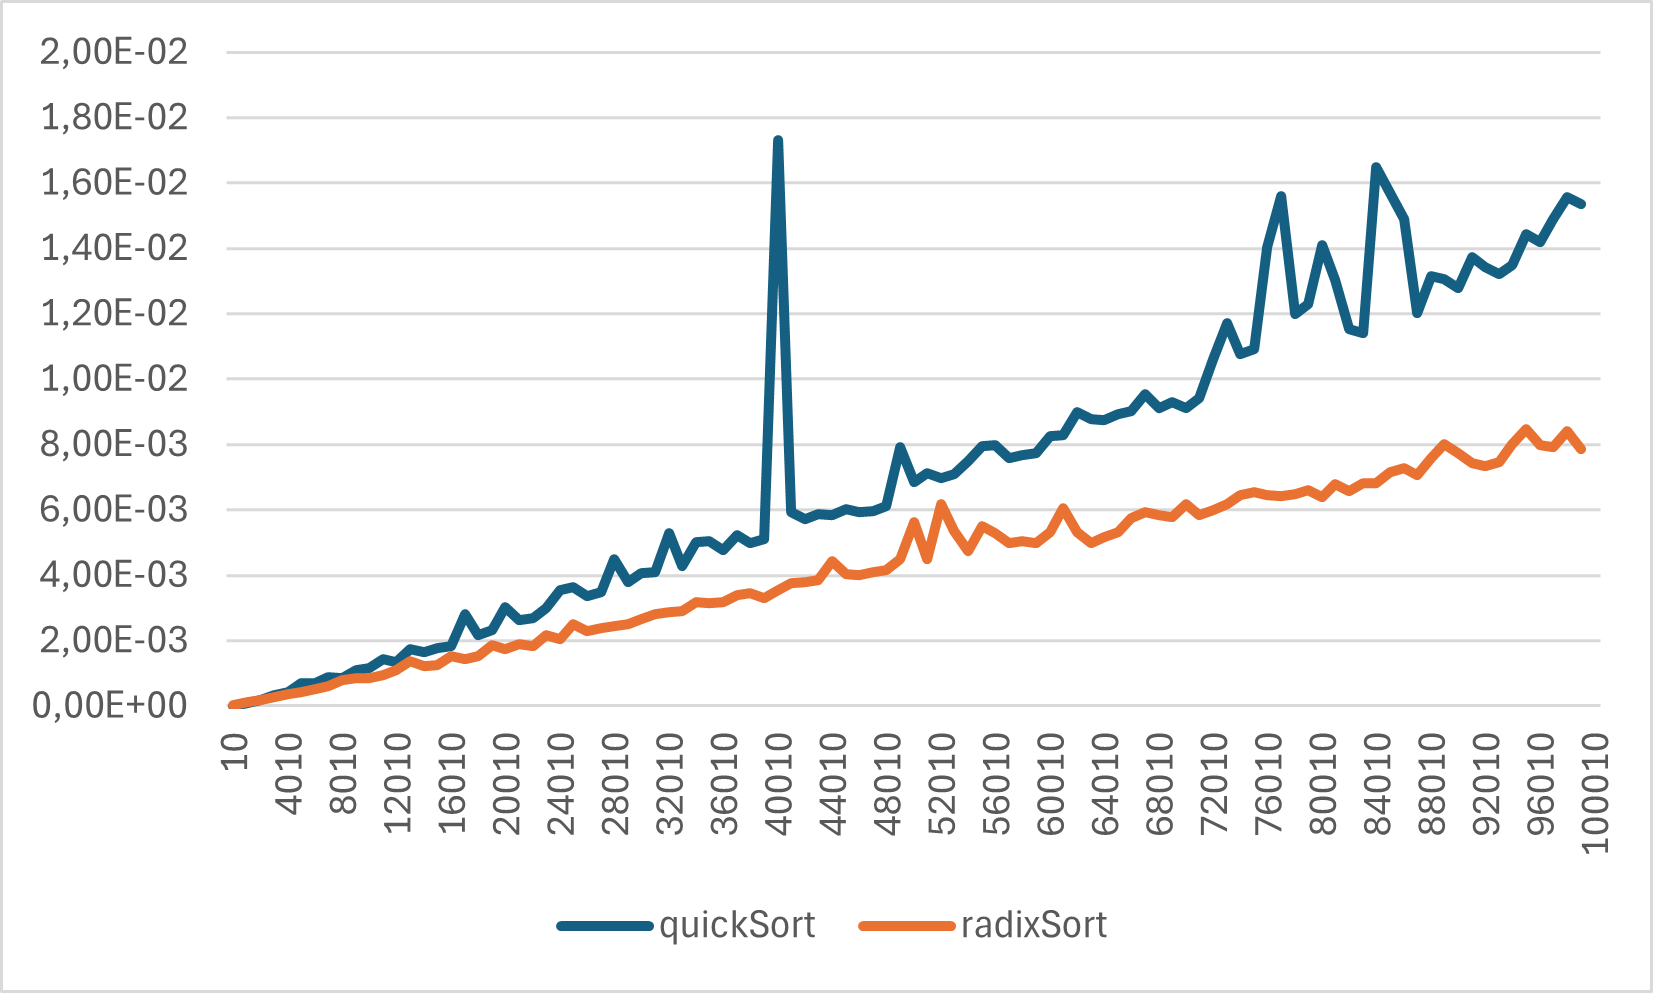
\includegraphics[width=\textwidth]{quickradix.png}
		\caption{Porównanie czasów działania \textit{quick sort} i \textit{radix sort}}
	\end{figure}
	Na wykresie możemy zobaczyć, że quick sort jak i radix sort mają bardzo podobne czasy działania, jest to spowodowane podobną złożonością obliczeniową, różnice są na poziomie stałej
	
	
	\section{Porównanie modyfikacji algorytmów}
	
	\subsection{\textit{Radix sort}}
	Zmodyfikowana wersja obsługuje liczby ujemne, dzieląc dane na dodatnie i ujemne, następnie ujemne zmienia na dodatnie, sortuje i w odwrotnej kolejności dodaje do pierwotnej tablicy wraz ze zmienionym znakiem
	\begin{lstlisting}
for(int i = 0; i<n; i++){ 
	if(A[i] < 0){
		U[j] = -A[i];
		j++;
	}else{
		D[l] = A[i];
		l++;
	} 
}

radixSort(D, l, baza);
radixSort(U, j, baza);
	\end{lstlisting}
	
	\begin{figure}[H]
		\centering
		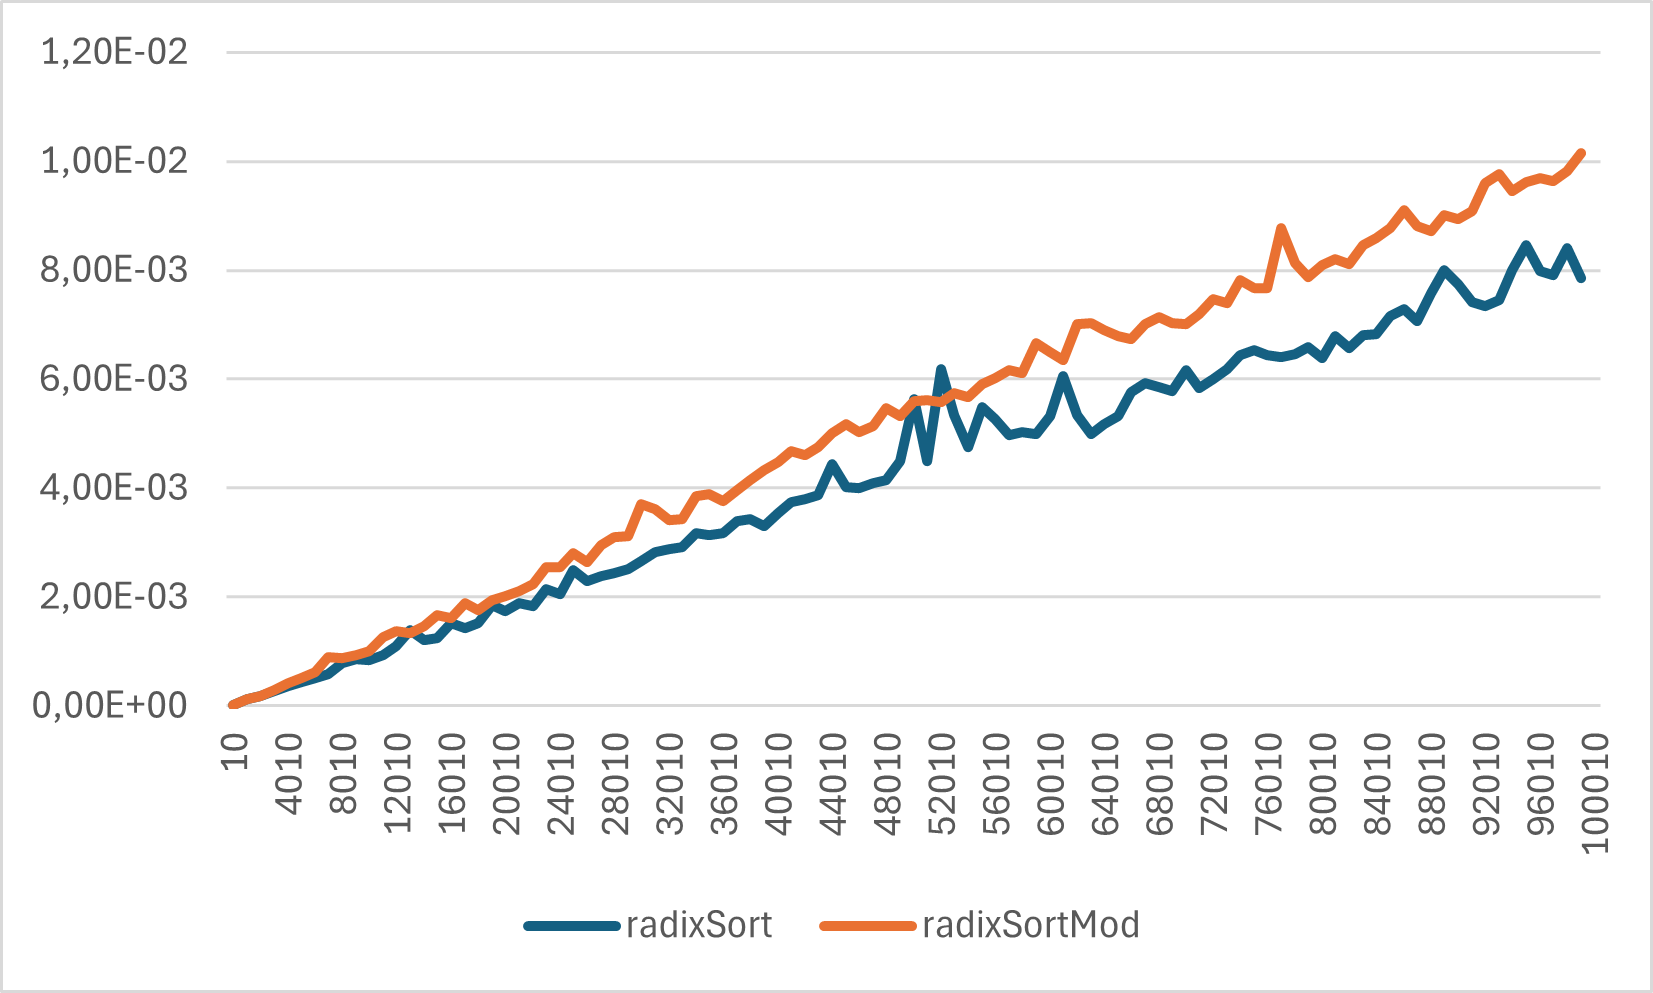
\includegraphics[width=\textwidth]{radix.png}
		\caption{Porównanie czasów działania \textit{radix sort} i jego modyfikacji}
	\end{figure}
	
	Dodanie obsługi liczb ujemnych zwiększa elastyczność algorytmu kosztem dodatkowej pamięci.
	
	
	\subsection{\textit{Quick sort}}
	Modyfikacja \textit{quick sort} polega na podziale tablicy za pomocą dwóch pivotów, a następnie rozdzieleniu na trzy części tablicy, tak jak jest to zrobione w poniższym kodzie:
	\begin{lstlisting}
		if (A[j] < x) {
			std::swap(A[i], A[j]);
			i++;
		} else if (A[j] > x2) {
			std::swap(A[k], A[j]);
			k--;
		}
	\end{lstlisting}
	
	\subsection{\textit{Bucket sort}}
	Zmodyfikowana wersja dynamicznie dopasowuje przedziały kubełków - normalizuje je tak, aby nie wypaść za przedział miedzy 0 a 1, nastepnie tak jak w oryginale, przypisuje do kubełków i sortuje wewnątrz:
	
	\begin{lstlisting}
int b = n * (A[i] - min) / (max - min);
	\end{lstlisting}
	
	\begin{figure}[H]
		\centering
		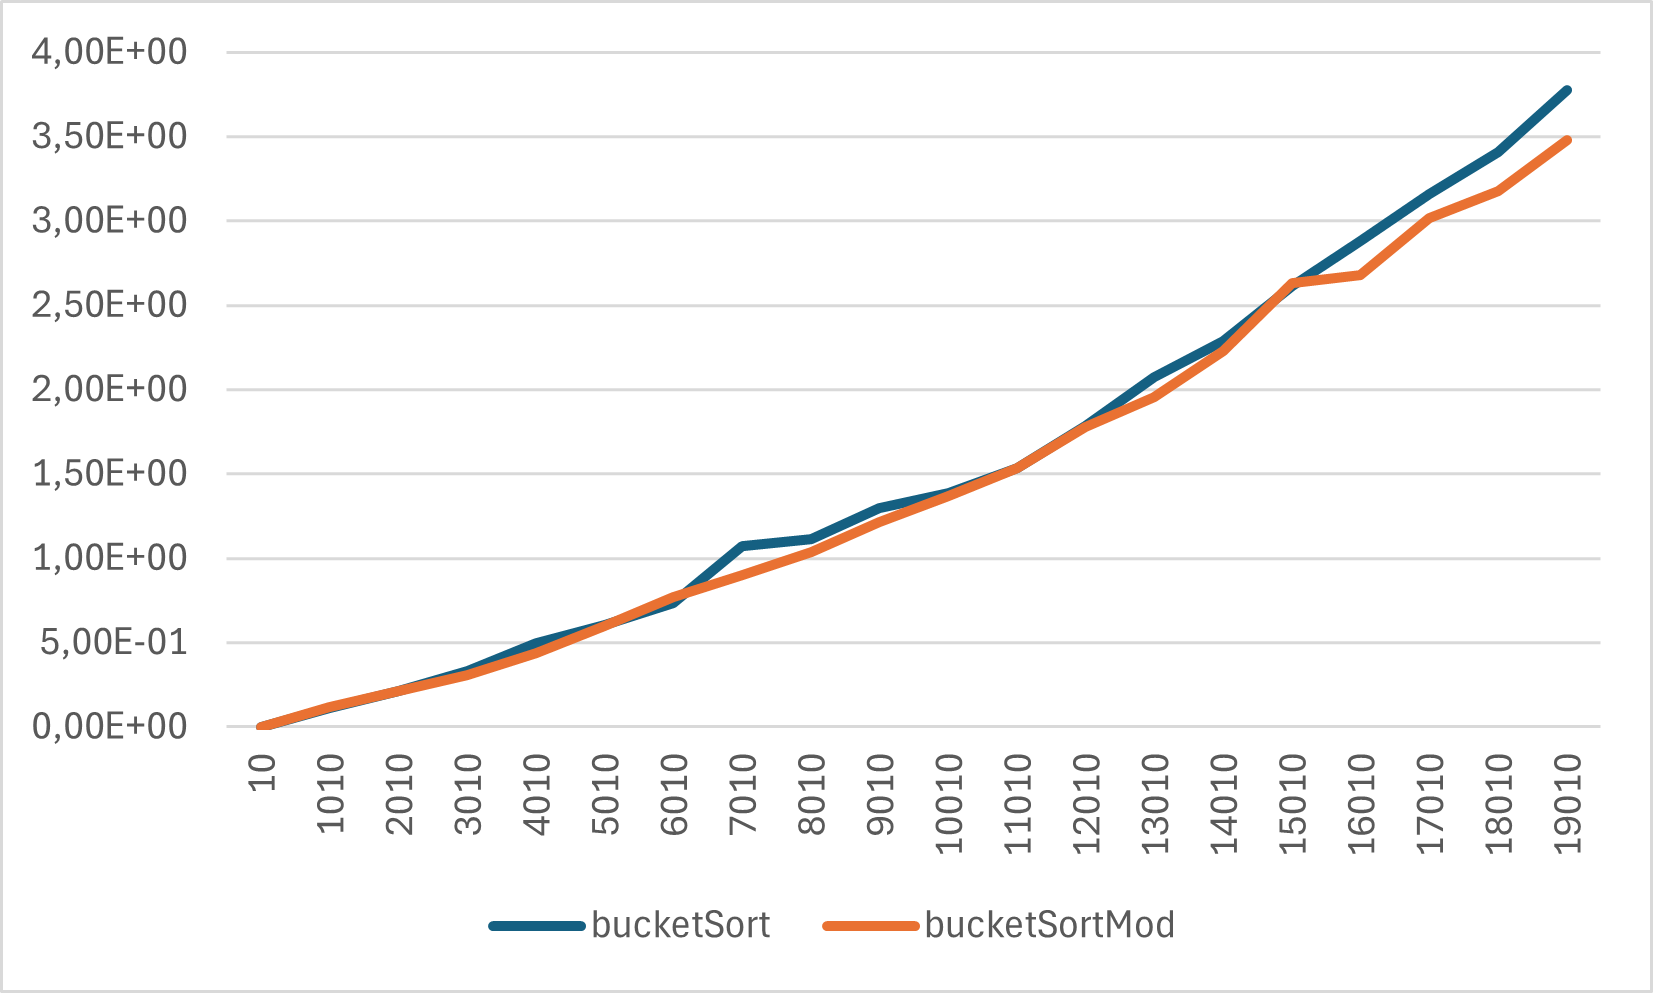
\includegraphics[width=\textwidth]{bucket.png}
		\caption{Porównanie czasów działania \textit{bucket sort} i jego modyfikacji}
	\end{figure}
	
	\section{\textit{Insertion sort} w listach jednokierunkowych}
	
	\subsection{Opis działania}
	Struktura listy jednokierunkowej została zainicjowana wraz z podaniem wartości:
	\begin{lstlisting}
SLel *L;     
SLel *e,* p; 
int n=6;
int values[] = {5, 2, 9, 1, 5, 6}; 
	\end{lstlisting}
	A następnie \textit{Insertion sort} szuka miejsca dla każdego elementu z $values$ a następnie wstawia w nie łącząc się z poprzednim oraz następnym miejscem:
	\begin{lstlisting}
for (p = L; v > p->next->data; p = p->next);
e = new SLel;
e->data = v;
e->next = p->next;
p->next = e;
	\end{lstlisting}
	Algorytm cechuje się prostotą implementacji, ale ma złożoność $O(n^2)$.
	
	\section{Wnioski}
	Przeprowadzone badania pokazują, że algorytmy \textit{radix sort} i \textit{bucket sort} są bardziej wydajne w scenariuszach z dużymi danymi. \textit{Quick sort} pozostaje uniwersalnym wyborem dzięki prostocie implementacji. Modyfikacje poprawiają działanie w specyficznych przypadkach, jednak kosztem większego skomplikowania kodu.
	
\end{document}
